\subsection{Sweep over disturbance magnitude}
\label{sec:scale}

Table~\ref{tab:scale} and Figure~\ref{fig:scale} report the sweep over \(\varphi\)
(\texttt{congested\_8x4x4}, \(\NSeeds\) random seeds; R0+ budget \(2\)\,s).
Per-level results are given in the table; R0+ still attains the better \(C_{\max}\) throughout, consistent with Section~\ref{sec:e5}.
On the small instance \texttt{example\_3x3x2}, every cell is likewise feasible (\(\NSeeds\) random seeds \(\times\) five
values of \(\varphi\)); bounded repair takes on the order of \(1\)\,ms,
and the time ratio ranges from \(\SpeedLo\times\) to \(\SpeedHi\times\) (per-cell extremes across both instances). The numerator of this ratio is the \emph{budget} of R0+ and the denominator is the measured wall-clock time of bounded repair. Since R0+ attains the better \(C_{\max}\),
the ratio should not be read as a speedup at equal solution quality.

Bounded repair in this section has scope escalation after failure enabled, so its results are not directly comparable with those of E3 and E5.
Even when the disturbance fraction reaches \(\varphi=1\) (all future operations disturbed), the runtime remains on the order of ten milliseconds and does not grow noticeably with the disturbance magnitude.
This runtime is due to single-pass rerouting (Section~\ref{sec:cheap}).

\begin{table}[t]
\centering
\caption{Comparison across disturbance magnitudes (\texttt{congested\_8x4x4}, averaged over \(\NSeeds\) random seeds).
Bounded repair includes scope escalation; R0+ budget \(2\)\,s. Dispersion is reported as the interquartile range: over the whole sweep, the STRC runtime ranges over
\ScaleMsMin--\ScaleMsMax\,ms, and the per-level IQR of the R0+ \(C_{\max}\) lies between \ScaleCmaxIqrLo\ and \ScaleCmaxIqrHi.
\textbf{At the two smallest levels, the within-level IQR of the ``Time ratio'' column exceeds the between-level variation of that column,
so the column indicates only the order of magnitude, not a trend in \(\varphi\).} The column gives the level mean of \emph{per-cell} ratios (paired first, then aggregated);
it therefore does not equal the ratio of the level means of the two adjacent columns. By the convexity of \(1/x\), the two generally differ, and recomputation should use the per-cell data.
The numerator is the wall-clock \emph{budget} of R0+, not its measured runtime, so this is not a comparison at equal quality (Section~\ref{sec:protocol}).}
\label{tab:scale}
\small
\begin{tabular}{@{}rcccc@{}}
\toprule
\(\varphi\) & STRC feasible & STRC\,ms & R0+ \(C_{\max}\) & Time ratio \\
\midrule
\(0.10\) & \(100\%\) & \(9.1\)  & \(103.5\) & \(406\times\) \\
\(0.25\) & \(100\%\) & \(11.1\) & \(107.0\) & \(325\times\) \\
\(0.50\) & \(100\%\) & \(8.6\)  & \(111.8\) & \(333\times\) \\
\(0.75\) & \(100\%\) & \(8.4\)  & \(125.8\) & \(254\times\) \\
\(1.00\) & \(100\%\) & \(10.7\) & \(148.1\) & \(203\times\) \\
\bottomrule
\end{tabular}
\end{table}

\begin{figure}[t]
\centering
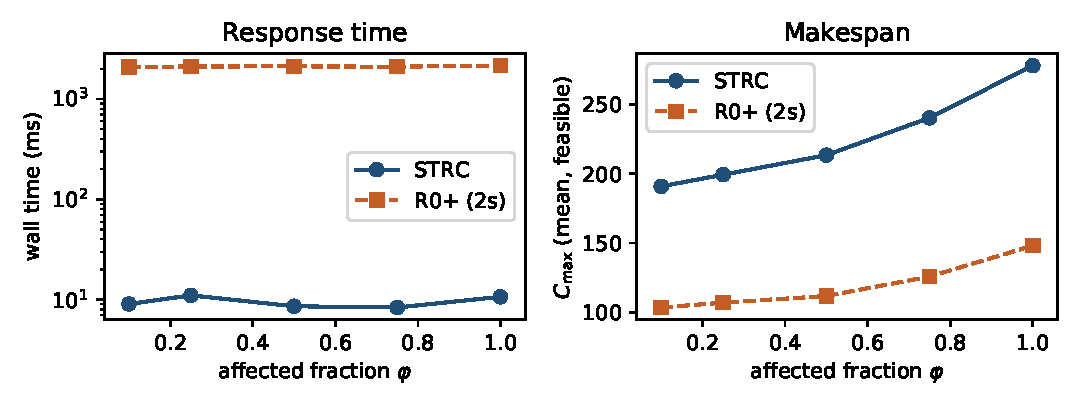
\includegraphics[width=\linewidth]{figures/fig_strc_scale}
\caption{Sweep over disturbance magnitude (\texttt{congested\_8x4x4}, \(\NSeeds\) random seeds):
runtime (log scale) and makespan of bounded repair and R0+ as functions of \(\varphi\). Curves show per-level means;
dispersion is measured as in Table~\ref{tab:scale} (interquartile range). On the runtime side, the range over the whole sweep is
\ScaleMsMin--\ScaleMsMax\,ms, always on the order of ten milliseconds; this is the only result on which the conclusion of this section rests.}
\Description{Two curves plotted against the disturbance fraction. Runtime is drawn on a logarithmic vertical axis: bounded repair stays on the order of
ten milliseconds and does not grow noticeably as the fraction increases, while global rescheduling stays fixed at the two-second budget line. On the makespan side,
global rescheduling rises slowly as the disturbance fraction increases, but remains below bounded repair throughout.}
\label{fig:scale}
\end{figure}

\subsection{E8: extrapolation to larger instances}
\label{sec:instscale}

The previous section swept the magnitude of the \emph{disturbance}, with the instance fixed at \(8\) jobs and \(4\) machines. This section turns to the other dimension: the disturbance protocol is fixed and
the instance itself is enlarged. The key question here is not runtime (runtime is expected not to grow noticeably) but \textbf{whether the impact-set share
approaches \(1\) as the instance grows, which would make ``bounded'' meaningless in practice}.

The size sequence uses \(2k\) jobs, \(k\) machines, and \(k\) vehicles for \(k=4,\dots,10\), that is, from \(8\times4\times4\) to
\(\ScaleJobsHi\times\ScaleMachHi\times\ScaleMachHi\): \(\ScaleKs\) levels \(\times\)
\(\NSeeds\) random seeds \(=\ScalePairs\) pairs. The congestion level, heterogeneity, flexibility, transport-to-processing time ratio, and the load/unload-station
minimum cut and remote cut are all calibrated to the same targets, so \emph{only the size changes}. The three baseline methods are defined as in Section~\ref{sec:cheap}.

\begin{table}[t]
\centering
\caption{E8 sweep over instance size (\(\ScaleKs\) levels \(\times\) \(\NSeeds\) random seeds).
``Impact set'' is the reservation impact set as a share of the \emph{whole table}; the attainable upper bound of this share is \(|R^{\circ}|/|R|\), whose mean in this batch is about
\ScaleAliveShare. With the rewritable set as the denominator, the share is \ScaleCloAliveLo--\ScaleCloAliveHi\ (see the text).
Runtimes are medians, and the ``RD/R2'' column is the \emph{ratio of the two median columns}. When the text discusses monotonicity, it uses level means of per-cell paired ratios;
the two measures rise and fall alike across levels but differ in value. The last column gives the win/tie/loss of R2 against RS on \(C_{\max}\).}
\label{tab:instscale}
\small
\begin{tabular}{@{}lrccccc@{}}
\toprule
Size & \(|R|\) & Impact set & R2\,ms & RD\,ms & RD/R2 & R2 vs.\ RS \\
\midrule
\(8\times4\times4\)    & \(148\) & \(0.561\) & \(2.9\)  & \(4.4\)  & \(1.5\times\) & \(7/1/2\) \\
\(10\times5\times5\)   & \(172\) & \(0.485\) & \(3.2\)  & \(6.1\)  & \(1.9\times\) & \(9/0/1\) \\
\(12\times6\times6\)   & \(230\) & \(0.481\) & \(4.5\)  & \(10.7\) & \(2.4\times\) & \(7/1/2\) \\
\(14\times7\times7\)   & \(281\) & \(0.492\) & \(6.1\)  & \(14.5\) & \(2.4\times\) & \(8/0/2\) \\
\(16\times8\times8\)   & \(291\) & \(0.534\) & \(6.4\)  & \(16.4\) & \(2.6\times\) & \(10/0/0\) \\
\(18\times9\times9\)   & \(356\) & \(0.535\) & \(8.2\)  & \(26.4\) & \(3.2\times\) & \(10/0/0\) \\
\(20\times10\times10\) & \(402\) & \(0.476\) & \(10.4\) & \(34.2\) & \(3.3\times\) & \(10/0/0\) \\
\bottomrule
\end{tabular}
\end{table}

Per-level results are given in Table~\ref{tab:instscale}.

\textbf{The impact-set share does not rise with instance size, but whether it ``approaches \(1\)'' can only be answered with the appropriate denominator.}
Across the seven levels, \(\mathrm{Cl}/|R|\) fluctuates between \ScaleCloLo\ and \ScaleCloHi\ without monotone trend
(highest at the first level, lowest at the last, and back above \(0.53\) at the fifth and sixth). Because \(\mathrm{Cl}\) contains only
occupancies that are unfinished after \(t_{\mathrm{now}}\), and the mean of \(|R^{\circ}|/|R|\) in this batch is only \ScaleAliveShare,
the attainable upper bound of \(\mathrm{Cl}/|R|\) is about \ScaleAliveShare, not \(1\). With the rewritable set as the denominator,
\(\mathrm{Cl}/|R^{\circ}|\) lies in \ScaleCloAliveLo--\ScaleCloAliveHi\ across the seven levels (per-cell maximum \(1.00\)),
the same order of magnitude as the \ClosureAliveFrac\ of the main batch in Sections~\ref{sec:e6} and~\ref{sec:cheap}.
This section therefore shows that \emph{the share does not rise with instance size}, but the impact set is not small relative to the rewritable set (Remark~\ref{rem:minimality}),
and seven levels are insufficient to support an asymptotic conclusion.

\textbf{Runtime grows faster than the total number of occupancies.} As \(|R|\) grows by a factor of \(2.7\), the median runtime of R2 grows from
\(2.9\)\,ms to \ScaleMsHi\,ms, a factor of \(3.6\), and remains on the order of ten milliseconds; seven levels are insufficient to determine the growth order. Level-1 rerouting is feasible in \ScaleFeasFirst\ cells.
The single failing cell (\(10\times5\times5\), random seed \(42\)) restored feasibility in round \(3\) of scope escalation after failure,
with a total runtime of \(12.0\)\,ms and the same makespan as the level-1 attempt; hence the final number of feasible cells is \ScaleFeasAll.

\textbf{The runtime gap between the two baseline methods widens with instance size.} The runtime ratio of the fastest global recomputation to bounded repair
rises from \ScaleRatioLo\(\times\) to \ScaleRatioHi\(\times\); that is, the larger the instance, the higher the runtime cost of global recomputation.
The per-level ratio is \emph{not monotone} (the level mean of per-cell paired ratios dips from \(k=6\to 7\)), but the two ends differ by \(1.8\),
far more than any within-level interquartile range (at most \(0.74\)); the \emph{overall rise} is therefore not noise.

Against the global right shift, which does not delineate the scope by the impact set, R2 has a \(C_{\max}\) win/tie/loss of \(10/0/0\) at each of the last three levels, while the first four levels
range between \(7\) and \(9\) wins with no monotone change; with only \NSeeds\ cells per level, no trend can be established.

\textbf{Scope of the evidence.} This size sequence covers a single congestion level and a single instance seed (every level's instance is generated from random seed
\(42\)), and tests only the dimension of \emph{size}; the sweeps of Sections~\ref{sec:e6} and~\ref{sec:scale} were not rerun on this batch.
In terms of contributions, this section adds evidence along the size dimension to the boundedness claim of C2: the share did not rise across these seven levels.

\subsection{Reproduction on the external-layout batch}
\label{sec:pubrepro}

For the second batch of Section~\ref{sec:protocol}, whose layouts are taken from an external source, the results of E1, E2, E3, and E5 on \(\NPubPairs\) instance--seed pairs
point \emph{in the same direction, item by item,} as those of the main batch:
the operation-precedence graph yields an empty scope in \PubPassMiss, structural containment (i.e., zero leaks) holds in \PubPassClosed,
and fields outside the set are unchanged entry by entry in \PubPassInvar. Under the boundary ablation, level-1 rerouting is feasible in \PubFeasRone\ cells when scoping on the operation-precedence graph and
in \PubFeasRtwo\ when scoping on the reservation impact set. Under the E1 protocol, the per-layout medians of the impact-set share lie in
\PubEoneFracLo--\PubEoneFracHi; the corresponding main-batch result is the pooled median over \NPairs\ pairs, \EoneFracMed\
(\EoneCloLo--\EoneCloHi\ is the range of per-instance \emph{means}, a different measure).
The external batch is slightly lower overall, but both are about one half, and the shortfall is of the same order as the variation across instances (figure caption in Section~\ref{sec:e1}).
The trade-off against global rescheduling is also unchanged: at \PubEfiveNoCross\ budget points R0+ attains the better \(C_{\max}\),
at the remaining \(1\) point the two methods tie (\texttt{LyuL6\_8m}, random seed \(2024\), budget \(0.2\)\,s), and at no point is R0+ worse.
This batch uses the same E5 code and the same parameters as the main batch, so Section~\ref{sec:e5} analyzes the two batches pooled over \(\EfiveCells\)
instance--seed cells; the tied cell also satisfies the monotonicity criterion of that section, and there is still no crossover.

This batch tests whether the above phenomena hold only on layouts designed by us. The results also hold on a batch of topologies not chosen by us,
so the object level of C1 and C2 does not depend on our layout design. The only conclusion this batch changes is the one on structural predictability (Section~\ref{sec:e4}).

\subsection{Summary}
\label{sec:exp_summary}

We group the results of this section by the contribution level they support; the limitations and the levels they affect are collected in Section~\ref{sec:limitations}.

\textbf{The object level} (C1, C2: on which object the scope is delineated, and whether the resulting set is uniquely determined) is supported by four groups of results.
Under corridor blockage, the scope on the operation-precedence graph is empty although the original schedule is indeed infeasible (E1, \(\PassMiss\) over \(\NPairs\) pairs).
The reservation impact set is closed under dependency edges, and fields outside the set are unchanged entry by entry (E2, \(\PassClosed\), \(\PassInvar\)).
With the same rerouting procedure and only the scope object changed, the feasibility rate goes from \(\FeasRone\) to \(\FeasRtwo\) (E3),
so feasibility depends on the scope object rather than on the quality of the rerouting procedure. Across four disturbance types crossed with two scope objects, the A/B dichotomy holds without exception,
and for Class A the reservation impact set always contains the scope obtained on the operation-precedence graph (E6).
Propositions~\ref{prop:miss}--\ref{prop:outside} give the corresponding structural statements,
with Proposition~\ref{prop:outside} still serving only as a sufficient condition.

\textbf{The net-benefit level} (C3: what this way of delineating the scope gains) is supported by a single group of results. Switching to a baseline that does not restrict the scope to the impact set
(RA, which uses the same rerouting as R2 and likewise does not rewrite finished occupancies) leaves runtime and \(C_{\max}\) almost unchanged,
yet raises the rewrite fraction from \ResFracCheapRtwo\ to \ResFracAllFuture\ (per cell \RAStabWTL, \(p=\RAStabP\);
Section~\ref{sec:cheap}). Hence the millisecond-scale response is due to single-pass rerouting rather than to the impact set, and
\textbf{the reduction in rewriting can be attributed only through this comparison}. Compared with warm-started global rescheduling, bounded repair is better on \(C_{\max}\)
in no cell, and relaxing the budget produces no crossover (E5); E7 rules out the explanation that the baseline methods simply ran too long.

The remaining results are qualifying results. The instance size has been extended to \(\ScaleJobsHi\) jobs and
\(\ScaleMachHi\) machines, and the impact-set share with the rewritable set as denominator did not rise with size (E8);
structural predictability is a negative result (E4). The second batch of instances (\(\NPubPairs\) pairs) only tests whether the above phenomena depend on
layouts designed by us, and the results of E1, E2, E3, and E5 are reproduced item by item.

%% =====================================================================
\section{Conclusion}
\label{sec:conclusion}
%% =====================================================================

This paper makes three contributions. \textbf{First} (C1), it identifies a class of failures that the operation-precedence graph cannot capture: corridor blockage changes no operation assignment,
so the scope delineated by affected operations is empty, although the original schedule is indeed infeasible (\(\PassMiss\) over \(\NPairs\) pairs, Section~\ref{sec:e1}).
\textbf{Second} (C2), it takes the reservation impact set obtained by \STRC as the rescheduling scope: once the dependency relations are given, whether an occupancy belongs to the set is
uniquely determined, and no dependency edge points from inside the set to outside it (\(\PassClosed\), \(\PassInvar\), Section~\ref{sec:e2}).
\textbf{Third} (C3), it provides a local recovery matched to this scope and separates the sources of the individual results: with the same rerouting procedure and only the scope object changed,
the feasibility rate goes from \(\FeasRone\) to \(\FeasRtwo\) (Section~\ref{sec:e3}),
so feasibility depends on the scope object rather than on the quality of the rerouting procedure.

Yielding relations, rerouting inside the set while keeping everything outside it as planned, and scope escalation after failure are all taken from the existing literature
(Section~\ref{sec:rw_claim}). Our claim is as follows.
By definition, the operation-precedence graph contains no yielding relations between corridor occupancies, and therefore cannot capture disturbances that invalidate only occupancies.
Once the scope is delineated on the reservation dependency graph, the occupancies that must be rewritten are uniquely determined by the given precedence relations, not by a heuristic radius.

If the rewritable set is changed from the reservation impact set to ``all occupancies unfinished after \(t_{\mathrm{now}}\)''
with all else unchanged, runtime and makespan remain almost the same, yet the rewrite fraction rises from \ResFracCheapRtwo\ to
\ResFracAllFuture\ (Section~\ref{sec:cheap}).
Hence the millisecond-scale response comes from single-pass rerouting without restarting the search; \textbf{the reduction in rewriting can be attributed only through this comparison,
and it reflects the property guaranteed by Proposition~\ref{prop:outside}: occupancies outside the set are kept as planned}.
The size of this benefit depends on how much smaller the impact set is than this trivial upper bound, and the benefit vanishes as the two approach each other.

\subsection{Limitations}
\label{sec:limitations}

The following four limitations are ordered by their impact on the preceding results; Section~\ref{sec:future} gives a direction for addressing each of them.

\begin{enumerate}[leftmargin=1.6em,itemsep=0.35em]
\item \textbf{The makespan is worse than that of warm-started global rescheduling that does not rewrite finished occupancies, and relaxing the budget produces no crossover.}
Bounded repair trades makespan for runtime, and over the \(\EfiveCells\) instance--seed cells tested, this disadvantage
does not reverse as the budget is relaxed (Section~\ref{sec:e5}).
This limitation concerns the net benefit of the scoping, not the object-level conclusions; the comparison of rewriting volume is given in Section~\ref{sec:cheap}.

\item \textbf{For the reservation impact set, the guarantee of Proposition~\ref{prop:outside} is only a sufficient condition; the dependency edge set has not been independently
and exhaustively verified; the rewritable set is not tight; and its size cannot be predicted by static indicators that depend only on the network.}
The impact set covers about \(\ClosureAliveFrac\) of the occupancies unfinished after \(t_{\mathrm{now}}\) (Remark~\ref{rem:minimality}).
The size of the net benefit depends on how much smaller the impact set is than this trivial upper bound, and the benefit vanishes as the two approach each other.
The family of static cut indicators has been ruled out in Section~\ref{sec:e4}, and the general relation between network geometry and impact-set size remains open.
This limitation concerns the strength and tightness of the object-level guarantee; it does not affect the diagnosis that scoping on the operation-precedence graph yields an empty scope.

\item \textbf{The implementation covers less than the problem scope described in the text: Class B disturbances are handled by rerouting only; Class A additionally allows vehicle swapping and reassignment
but no change of processing order; and, by Assumption A3, only a single response is made.}
Opening up the processing order degenerates into global rescheduling, at which point ``bounded'' loses its meaning; disturbance streams, prediction errors, and rolling responses are not addressed.
The size dimension has been extended to \(\ScaleJobsHi\) jobs and \(\ScaleMachHi\) machines without the impact-set share rising with size,
but the number of levels swept is insufficient to support asymptotic claims. This limitation restricts extrapolation of the results to larger instances and to continual disturbances.

\item \textbf{External reference points are lacking: this line of research has no public benchmark that can be substituted in, the provenance of the instances is externalized only at the topology level,
and the results have not been reproduced on a second implementation.}
The public instance families~\cite{homayouni2021production,bilge1995time} publish transport times as machine-to-machine travel-time matrices rather than as networks. We checked all \(11\) layouts of the two families one by one, and none of them
can be reconstructed as an undirected corridor graph consistent with the published matrix; hence \(R\), \(G_R\), \(\mathrm{Cl}(\cdot)\), and Class B disturbances
cannot be defined on them (Section~\ref{sec:protocol}).
The second batch of instances is built from the appendix layouts of Lyu et al.~\cite{lyu2019approach}, so the layouts are no longer designed by us.
However, the per-leg travel times and job data are still our own, so the batch cannot be used to reproduce the reference values of Lyu et al.\ or van Os~\cite{vanos2026exact},
and its coverage is also smaller than that of the main batch. This limitation concerns external validity; the relative results among baselines within the same implementation are unaffected.
\end{enumerate}

\subsection{Future work}
\label{sec:future}

The following four directions correspond one to one to the four limitations of the previous section.

\textbf{1. Narrowing the makespan gap} (Limitation \(1\)).
In the main batch, prefix decoding does not rewrite finished occupancies (the number of violations over the \(18\) budget points of E5 is \(\RzeroPastLo\),
and that of RD on E7 is \RedecodeBad), so Limitation 1 concerns only \(C_{\max}\) itself.
Narrowing the gap would require limited reassignment or resequencing without rewriting finished occupancies, but this would make the method degenerate toward global rescheduling.

\textbf{2. Making the guarantee of the reservation impact set more complete and tighter, and characterizing its size} (Limitation \(2\)).
\emph{Completeness}: under the current yield edge set, the leakage found by the probe is \ProbeLeaks.
The next step is to probe with other disturbance forms (e.g., shortening occupancies, or delaying them by more than \(1\) time unit), rather than to keep adding dependency edges of the same kind.
\emph{Tightness} points to a minimal rewritable set: define minimality for a fixed repair capability
and quantify the gap between the impact set and it. This is a necessary step to advance ``bounded'' from a sufficient condition to a tight bound; the current impact set covers about
\(\ClosureAliveFrac\) of the unfinished occupancies, so the gap may be considerable. \emph{Size characterization} currently has only one
post hoc rule (the rewritable share, Figure~\ref{fig:worth}), but it varies with the schedule, and an indicator computable before the disturbance is needed instead.
Section~\ref{sec:e4} has ruled out the family of static cut indicators: they are constant on practical layouts, whereas on the same network
merely changing the machine configuration changes the impact-set share. On the \(4\times 4\) network, going from \(4\) to \(5\) machines changes it by \PubCloSpread;
on the \(5\times 5\) network, the three configurations (\(6\), \(7\), and \(8\) machines) differ by \PubCloSpreadBig.
This suggests that what matters may be the \emph{spatial distribution of demand}, rather than the traffic capacity the network provides.
The next candidate is the temporal density of corridor occupancies in the neighborhood of \(t_{\mathrm{now}}\), for example the number of
overlapping occupancies on the disturbed corridor within its busy window, and the out-degree of that corridor in the yielding graph. Such quantities vary with the schedule and are no longer purely topological,
so the notion of ``predictability'' must accordingly be restated as predicting the size from a given layout \emph{and the current schedule}.

\textbf{3. Relaxing Assumption A3} (Limitation \(3\); A3 stipulates a single, fully observed disturbance).
The next step is not to open up resequencing further but to relax this assumption, examining whether the impact set accumulates and inflates under continual disturbances,
and whether an explicit ``restoration'' step is needed between two repairs.

\textbf{4. Taking the time calibration from an external source as well} (Limitation \(4\)). The layouts already come from an external source; for the time calibration,
an instance family that publishes both \emph{a network of exclusive corridors and per-leg durations} is still needed, and a self-built sweep over edge weights cannot substitute for it.
A second independent implementation need not be undertaken separately; it can be carried out together with reproducing any of the items above.

%% Standard back-matter: funding, acknowledgments, and conflict-of-interest statements are included as journals customarily require.
%% The acmart acks environment is hidden automatically in review/anonymous mode, so no manual removal is needed for anonymous submission.
\begin{acks}
This work was supported by <TO BE FILLED: funding program name and grant number>.
The authors thank the anonymous reviewers for their comments on the experimental measures and the boundaries of the conclusions.
\end{acks}

\section*{Conflict of interest statement}
The authors declare no conflicts of interest related to this work.

\bibliographystyle{ACM-Reference-Format}
\bibliography{reference-base}

\end{document}
